\chapter{The Hand of God}

Caderousse continued to call piteously, “Help, reverend sir, help!”

“What is the matter?” asked Monte Cristo.

“Help,” cried Caderousse; “I am murdered!”

“We are here;—take courage.”

“Ah, it’s all over! You are come too late—you are come to see me die.
What blows, what blood!”

He fainted. Ali and his master conveyed the wounded man into a room.
Monte Cristo motioned to Ali to undress him, and he then examined his
dreadful wounds.

“My God!” he exclaimed, “thy vengeance is sometimes delayed, but only
that it may fall the more effectually.” Ali looked at his master for
further instructions. “Bring here immediately the king’s attorney, M.
de Villefort, who lives in the Faubourg Saint-Honoré. As you pass the
lodge, wake the porter, and send him for a surgeon.”

Ali obeyed, leaving the abbé alone with Caderousse, who had not yet
revived.

When the wretched man again opened his eyes, the count looked at him
with a mournful expression of pity, and his lips moved as if in prayer.
“A surgeon, reverend sir—a surgeon!” said Caderousse.

“I have sent for one,” replied the abbé.

“I know he cannot save my life, but he may strengthen me to give my
evidence.”

“Against whom?”

“Against my murderer.”

“Did you recognize him?”

“Yes; it was Benedetto.”

“The young Corsican?”

“Himself.”

“Your comrade?”

“Yes. After giving me the plan of this house, doubtless hoping I should
kill the count and he thus become his heir, or that the count would
kill me and I should be out of his way, he waylaid me, and has murdered
me.”

“I have also sent for the procureur.”

“He will not come in time; I feel my life fast ebbing.”

“Wait a moment,” said Monte Cristo. He left the room, and returned in
five minutes with a phial. The dying man’s eyes were all the time
riveted on the door, through which he hoped succor would arrive.

“Hasten, reverend sir, hasten! I shall faint again!” Monte Cristo
approached, and dropped on his purple lips three or four drops of the
contents of the phial. Caderousse drew a deep breath. “Oh,” said he,
“that is life to me; more, more!”

“Two drops more would kill you,” replied the abbé.

“Oh, send for someone to whom I can denounce the wretch!”

“Shall I write your deposition? You can sign it.”

“Yes, yes,” said Caderousse; and his eyes glistened at the thought of
this posthumous revenge. Monte Cristo wrote:

\begin{quote}
{\small“I die, murdered by the Corsican Benedetto, my comrade in the galleys
at Toulon, No. 59.”}
\end{quote}

“Quick, quick!” said Caderousse, “or I shall be unable to sign it.”

Monte Cristo gave the pen to Caderousse, who collected all his
strength, signed it, and fell back on his bed, saying:

“You will relate all the rest, reverend sir; you will say he calls
himself Andrea Cavalcanti. He lodges at the Hôtel des Princes. Oh, I am
dying!” He again fainted. The abbé made him smell the contents of the
phial, and he again opened his eyes. His desire for revenge had not
forsaken him.

“Ah, you will tell all I have said, will you not, reverend sir?”

“Yes, and much more.”

“What more will you say?”

“I will say he had doubtless given you the plan of this house, in the
hope the count would kill you. I will say, likewise, he had apprised
the count, by a note, of your intention, and, the count being absent, I
read the note and sat up to await you.”

“And he will be guillotined, will he not?” said Caderousse. “Promise me
that, and I will die with that hope.”

“I will say,” continued the count, “that he followed and watched you
the whole time, and when he saw you leave the house, ran to the angle
of the wall to conceal himself.”

“Did you see all that?”

“Remember my words: ‘If you return home safely, I shall believe God has
forgiven you, and I will forgive you also.’”

“And you did not warn me!” cried Caderousse, raising himself on his
elbows. “You knew I should be killed on leaving this house, and did not
warn me!”

\begin{figure}[ht]
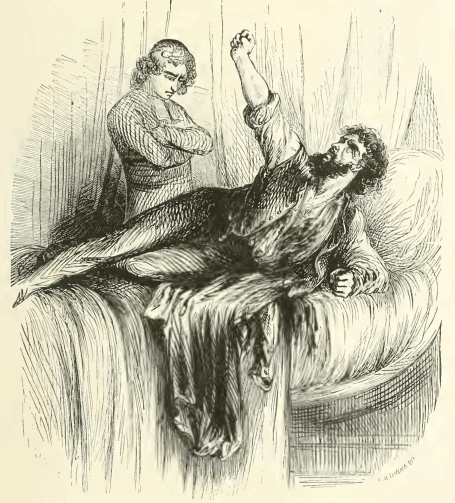
\includegraphics[width=\textwidth]{40168m.jpg}
\end{figure}

“No; for I saw God’s justice placed in the hands of Benedetto, and
should have thought it sacrilege to oppose the designs of Providence.”

“God’s justice! Speak not of it, reverend sir. If God were just, you
know how many would be punished who now escape.”

“Patience,” said the abbé, in a tone which made the dying man shudder;
“have patience!”

Caderousse looked at him with amazement.

“Besides,” said the abbé, “God is merciful to all, as he has been to
you; he is first a father, then a judge.”

“Do you then believe in God?” said Caderousse.

“Had I been so unhappy as not to believe in him until now,” said Monte
Cristo, “I must believe on seeing you.”

Caderousse raised his clenched hands towards heaven.

“Listen,” said the abbé, extending his hand over the wounded man, as if
to command him to believe; “this is what the God in whom, on your
death-bed, you refuse to believe, has done for you—he gave you health,
strength, regular employment, even friends—a life, in fact, which a man
might enjoy with a calm conscience. Instead of improving these gifts,
rarely granted so abundantly, this has been your course—you have given
yourself up to sloth and drunkenness, and in a fit of intoxication have
ruined your best friend.”

“Help!” cried Caderousse; “I require a surgeon, not a priest; perhaps I
am not mortally wounded—I may not die; perhaps they can yet save my
life.”

“Your wounds are so far mortal that, without the three drops I gave
you, you would now be dead. Listen, then.”

“Ah,” murmured Caderousse, “what a strange priest you are; you drive
the dying to despair, instead of consoling them.”

“Listen,” continued the abbé. “When you had betrayed your friend, God
began not to strike, but to warn you. Poverty overtook you. You had
already passed half your life in coveting that which you might have
honorably acquired; and already you contemplated crime under the excuse
of want, when God worked a miracle in your behalf, sending you, by my
hands, a fortune—brilliant, indeed, for you, who had never possessed
any. But this unexpected, unhoped-for, unheard-of fortune sufficed you
no longer when you once possessed it; you wished to double it, and
how?—by a murder! You succeeded, and then God snatched it from you, and
brought you to justice.”

“It was not I who wished to kill the Jew,” said Caderousse; “it was La
Carconte.”

“Yes,” said Monte Cristo, “and God,—I cannot say in justice, for his
justice would have slain you,—but God, in his mercy, spared your life.”

“\textit{Pardieu!} to transport me for life, how merciful!”

“You thought it a mercy then, miserable wretch! The coward who feared
death rejoiced at perpetual disgrace; for like all galley-slaves, you
said, ‘I may escape from prison, I cannot from the grave.’ And you said
truly; the way was opened for you unexpectedly. An Englishman visited
Toulon, who had vowed to rescue two men from infamy, and his choice
fell on you and your companion. You received a second fortune, money
and tranquillity were restored to you, and you, who had been condemned
to a felon’s life, might live as other men. Then, wretched creature,
then you tempted God a third time. ‘I have not enough,’ you said, when
you had more than you before possessed, and you committed a third
crime, without reason, without excuse. God is wearied; he has punished
you.”

Caderousse was fast sinking. “Give me drink,” said he: “I thirst—I
burn!” Monte Cristo gave him a glass of water. “And yet that villain,
Benedetto, will escape!”

“No one, I tell you, will escape; Benedetto will be punished.”

“Then, you, too, will be punished, for you did not do your duty as a
priest—you should have prevented Benedetto from killing me.”

“I?” said the count, with a smile which petrified the dying man, “when
you had just broken your knife against the coat of mail which protected
my breast! Yet perhaps if I had found you humble and penitent, I might
have prevented Benedetto from killing you; but I found you proud and
blood-thirsty, and I left you in the hands of God.”

“I do not believe there is a God,” howled Caderousse; “you do not
believe it; you lie—you lie!”

“Silence,” said the abbé; “you will force the last drop of blood from
your veins. What! you do not believe in God when he is striking you
dead? you will not believe in him, who requires but a prayer, a word, a
tear, and he will forgive? God, who might have directed the assassin’s
dagger so as to end your career in a moment, has given you this quarter
of an hour for repentance. Reflect, then, wretched man, and repent.”

“No,” said Caderousse, “no; I will not repent. There is no God; there
is no Providence—all comes by chance.”

“There is a Providence; there is a God,” said Monte Cristo, “of whom
you are a striking proof, as you lie in utter despair, denying him,
while I stand before you, rich, happy, safe and entreating that God in
whom you endeavor not to believe, while in your heart you still believe
in him.”

“But who are you, then?” asked Caderousse, fixing his dying eyes on the
count.

“Look well at me!” said Monte Cristo, putting the light near his face.

“Well, the abbé—the Abbé Busoni.” Monte Cristo took off the wig which
disfigured him, and let fall his black hair, which added so much to the
beauty of his pallid features.

“Oh?” said Caderousse, thunderstruck, “but for that black hair, I
should say you were the Englishman, Lord Wilmore.”

“I am neither the Abbé Busoni nor Lord Wilmore,” said Monte Cristo;
“think again,—do you not recollect me?”

There was a magic effect in the count’s words, which once more revived
the exhausted powers of the miserable man.

“Yes, indeed,” said he; “I think I have seen you and known you
formerly.”

“Yes, Caderousse, you have seen me; you knew me once.”

“Who, then, are you? and why, if you knew me, do you let me die?”

“Because nothing can save you; your wounds are mortal. Had it been
possible to save you, I should have considered it another proof of
God’s mercy, and I would again have endeavored to restore you, I swear
by my father’s tomb.”

“By your father’s tomb!” said Caderousse, supported by a supernatural
power, and half-raising himself to see more distinctly the man who had
just taken the oath which all men hold sacred; “who, then, are you?”

The count had watched the approach of death. He knew this was the last
struggle. He approached the dying man, and, leaning over him with a
calm and melancholy look, he whispered, “I am—I am——”

And his almost closed lips uttered a name so low that the count himself
appeared afraid to hear it. Caderousse, who had raised himself on his
knees, and stretched out his arm, tried to draw back, then clasping his
hands, and raising them with a desperate effort, “Oh, my God, my God!”
said he, “pardon me for having denied thee; thou dost exist, thou art
indeed man’s father in heaven, and his judge on earth. My God, my Lord,
I have long despised thee! Pardon me, my God; receive me, Oh, my Lord!”

Caderousse sighed deeply, and fell back with a groan. The blood no
longer flowed from his wounds. He was dead.

“\textit{One!}” said the count mysteriously, his eyes fixed on the corpse,
disfigured by so awful a death.

Ten minutes afterwards the surgeon and the procureur arrived, the one
accompanied by the porter, the other by Ali, and were received by the
Abbé Busoni, who was praying by the side of the corpse.
